\documentclass[12pt,]{article}
\usepackage{lmodern}
\usepackage{amssymb,amsmath}
\usepackage{ifxetex,ifluatex}
\usepackage{fixltx2e} % provides \textsubscript
\ifnum 0\ifxetex 1\fi\ifluatex 1\fi=0 % if pdftex
  \usepackage[T1]{fontenc}
  \usepackage[utf8]{inputenc}
\else % if luatex or xelatex
  \ifxetex
    \usepackage{mathspec}
  \else
    \usepackage{fontspec}
  \fi
  \defaultfontfeatures{Ligatures=TeX,Scale=MatchLowercase}
  \newcommand{\euro}{€}
\fi
% use upquote if available, for straight quotes in verbatim environments
\IfFileExists{upquote.sty}{\usepackage{upquote}}{}
% use microtype if available
\IfFileExists{microtype.sty}{%
\usepackage{microtype}
\UseMicrotypeSet[protrusion]{basicmath} % disable protrusion for tt fonts
}{}
\usepackage[margin=1in]{geometry}
\usepackage{hyperref}
\PassOptionsToPackage{usenames,dvipsnames}{color} % color is loaded by hyperref
\hypersetup{unicode=true,
            pdftitle={Data Analysis with Topic Models for Communications Researchers},
            pdfborder={0 0 0},
            breaklinks=true}
\urlstyle{same}  % don't use monospace font for urls
\usepackage{color}
\usepackage{fancyvrb}
\newcommand{\VerbBar}{|}
\newcommand{\VERB}{\Verb[commandchars=\\\{\}]}
\DefineVerbatimEnvironment{Highlighting}{Verbatim}{commandchars=\\\{\}}
% Add ',fontsize=\small' for more characters per line
\usepackage{framed}
\definecolor{shadecolor}{RGB}{248,248,248}
\newenvironment{Shaded}{\begin{snugshade}}{\end{snugshade}}
\newcommand{\KeywordTok}[1]{\textcolor[rgb]{0.13,0.29,0.53}{\textbf{{#1}}}}
\newcommand{\DataTypeTok}[1]{\textcolor[rgb]{0.13,0.29,0.53}{{#1}}}
\newcommand{\DecValTok}[1]{\textcolor[rgb]{0.00,0.00,0.81}{{#1}}}
\newcommand{\BaseNTok}[1]{\textcolor[rgb]{0.00,0.00,0.81}{{#1}}}
\newcommand{\FloatTok}[1]{\textcolor[rgb]{0.00,0.00,0.81}{{#1}}}
\newcommand{\ConstantTok}[1]{\textcolor[rgb]{0.00,0.00,0.00}{{#1}}}
\newcommand{\CharTok}[1]{\textcolor[rgb]{0.31,0.60,0.02}{{#1}}}
\newcommand{\SpecialCharTok}[1]{\textcolor[rgb]{0.00,0.00,0.00}{{#1}}}
\newcommand{\StringTok}[1]{\textcolor[rgb]{0.31,0.60,0.02}{{#1}}}
\newcommand{\VerbatimStringTok}[1]{\textcolor[rgb]{0.31,0.60,0.02}{{#1}}}
\newcommand{\SpecialStringTok}[1]{\textcolor[rgb]{0.31,0.60,0.02}{{#1}}}
\newcommand{\ImportTok}[1]{{#1}}
\newcommand{\CommentTok}[1]{\textcolor[rgb]{0.56,0.35,0.01}{\textit{{#1}}}}
\newcommand{\DocumentationTok}[1]{\textcolor[rgb]{0.56,0.35,0.01}{\textbf{\textit{{#1}}}}}
\newcommand{\AnnotationTok}[1]{\textcolor[rgb]{0.56,0.35,0.01}{\textbf{\textit{{#1}}}}}
\newcommand{\CommentVarTok}[1]{\textcolor[rgb]{0.56,0.35,0.01}{\textbf{\textit{{#1}}}}}
\newcommand{\OtherTok}[1]{\textcolor[rgb]{0.56,0.35,0.01}{{#1}}}
\newcommand{\FunctionTok}[1]{\textcolor[rgb]{0.00,0.00,0.00}{{#1}}}
\newcommand{\VariableTok}[1]{\textcolor[rgb]{0.00,0.00,0.00}{{#1}}}
\newcommand{\ControlFlowTok}[1]{\textcolor[rgb]{0.13,0.29,0.53}{\textbf{{#1}}}}
\newcommand{\OperatorTok}[1]{\textcolor[rgb]{0.81,0.36,0.00}{\textbf{{#1}}}}
\newcommand{\BuiltInTok}[1]{{#1}}
\newcommand{\ExtensionTok}[1]{{#1}}
\newcommand{\PreprocessorTok}[1]{\textcolor[rgb]{0.56,0.35,0.01}{\textit{{#1}}}}
\newcommand{\AttributeTok}[1]{\textcolor[rgb]{0.77,0.63,0.00}{{#1}}}
\newcommand{\RegionMarkerTok}[1]{{#1}}
\newcommand{\InformationTok}[1]{\textcolor[rgb]{0.56,0.35,0.01}{\textbf{\textit{{#1}}}}}
\newcommand{\WarningTok}[1]{\textcolor[rgb]{0.56,0.35,0.01}{\textbf{\textit{{#1}}}}}
\newcommand{\AlertTok}[1]{\textcolor[rgb]{0.94,0.16,0.16}{{#1}}}
\newcommand{\ErrorTok}[1]{\textcolor[rgb]{0.64,0.00,0.00}{\textbf{{#1}}}}
\newcommand{\NormalTok}[1]{{#1}}
\usepackage{graphicx,grffile}
\makeatletter
\def\maxwidth{\ifdim\Gin@nat@width>\linewidth\linewidth\else\Gin@nat@width\fi}
\def\maxheight{\ifdim\Gin@nat@height>\textheight\textheight\else\Gin@nat@height\fi}
\makeatother
% Scale images if necessary, so that they will not overflow the page
% margins by default, and it is still possible to overwrite the defaults
% using explicit options in \includegraphics[width, height, ...]{}
\setkeys{Gin}{width=\maxwidth,height=\maxheight,keepaspectratio}
\setlength{\parindent}{0pt}
\setlength{\parskip}{6pt plus 2pt minus 1pt}
\setlength{\emergencystretch}{3em}  % prevent overfull lines
\providecommand{\tightlist}{%
  \setlength{\itemsep}{0pt}\setlength{\parskip}{0pt}}
\setcounter{secnumdepth}{5}

%%% Use protect on footnotes to avoid problems with footnotes in titles
\let\rmarkdownfootnote\footnote%
\def\footnote{\protect\rmarkdownfootnote}

%%% Change title format to be more compact
\usepackage{titling}

% Create subtitle command for use in maketitle
\newcommand{\subtitle}[1]{
  \posttitle{
    \begin{center}\large#1\end{center}
    }
}

\setlength{\droptitle}{-2em}
  \title{Data Analysis with Topic Models for Communications Researchers}
  \pretitle{\vspace{\droptitle}\centering\huge}
  \posttitle{\par}
  \author{}
  \preauthor{}\postauthor{}
  \date{}
  \predate{}\postdate{}


\usepackage{setspace}
\doublespacing
\usepackage[nomarkers,figuresonly]{endfloat}
\usepackage[colorinlistoftodos]{todonotes}
\usepackage{ifthen}

% \usepackage[top=10mm, bottom=10mm, left=10mm, right=10mm,includehead,includefoot]{geometry}

\usepackage{fancyhdr}
\pagestyle{fancy}
\lhead{}
\chead{Data Analysis with Topic Models for Communications Researchers}
\rhead{}

% Redefines (sub)paragraphs to behave more like sections
\ifx\paragraph\undefined\else
\let\oldparagraph\paragraph
\renewcommand{\paragraph}[1]{\oldparagraph{#1}\mbox{}}
\fi
\ifx\subparagraph\undefined\else
\let\oldsubparagraph\subparagraph
\renewcommand{\subparagraph}[1]{\oldsubparagraph{#1}\mbox{}}
\fi

\begin{document}
\maketitle

\pagestyle{fancy}

\section{Abstract}\label{abstract}

We present a non-technical introduction to data analysis with topic
models for communications researchers. We motivate the discussion with a
research question from social media communications research. We then
discuss statistical aspects of topic models as we illustrate these
methods with data from The New York Times. We complement our discussion
with computer code (in the R computing language) that implements our
methods. We close with thoughts about the future value of topic modeling
to communications researchers.

\section{Motivation}\label{motivation}

We are in the big data era. Social media users inundate us with status
updates and tweets, while bloggers share their views on current events.
These new media interact with more established media, such as print news
media, television, and radio. What do they have in common? One answer is
that they all can be viewed as data sources in which words - whether
written or spoken, tweeted or blogged - are the data.

Think about how we currently browse this data. Let's suppose that we
want to read about mass shootings. We might search for the key words
``mass'' and ``shooting''. Doing so, we will find some articles that
deal with mass shootings, but other results may deal with other types of
``shootings'', such as film shooting or accidental shooting. Even if we
specify that the two-word phrase ``mass shooting'' must appear in our
results, we will find some articles that merely mention mass shootings,
and we'll miss relevant articles that don't explicitly use the term
``mass shooting''.

D. M. Blei (2012) envisions an alternative search strategy in which we
search for articles that are \emph{about} ``mass shootings''. Some of
the resulting articles would have the phrase ``mass shooting'', but
containing that two-word phrase is not required; the sole requirement is
that the article focus on mass shootings. That is, we'd like to see all
of the articles that have the theme, or ``topic'', mass shooting. Topic
modeling is one method that may ultimately enable us to do the
theme-based browsing that D. M. Blei (2012) suggests.

``Topic modeling'' refers to a collection of statistical and machine
learning methods that have the goal of discovering latent topics in a
large collection, or ``corpus'', of texts. The tremendous rise in
computing speed and memory capacity, coupled with the increasing
availability of digitized texts, has enabled researchers working at the
interface of quantitative methods and social sciences to treat written
texts as data.

While data analysis of documents is still in its infancy, scientists
nevertheless have made great progress towards computational dissection
and interpretation of texts. We detail below, with limited use of
statistical terminology, how these methods work and why they may be
useful in communications research. We illustrate topic modeling methods
in the analysis of all New York Times articles from three days in March
2016. We also provide an appendix with computer code (in the R computer
programming language) that implements these methods.

\section{Background}\label{background}

LDA is an extension of an earlier text analysis method called
``probabilistic latent semantic analysis'' (pLSA) (Hofmann, 1999).
Hofmann (1999) described pLSA as a ``latent class model for factor
analysis of count data''. The novelty of LDA, compared to pLSA, is that
LDA places a Dirichlet prior on the probability distributions of words.
This use of a Dirichlet prior makes computations convenient because of a
Bayesian statistical concept called ``conjugacy''. That is, the
posterior probability distribution, which is the object of statistical
inference, is also a Dirichlet distribution.

In the 13 years since the publication of D. M. Blei, Ng, \& Jordan
(2003), researchers have developed a wide variety of extensions to LDA.
Many of these extensions of LDA accommodate relationships among topics.
Widely used extensions of LDA include correlated topic models (D. M.
Blei \& Lafferty, 2007), hierarchical topic models (D. Griffiths \&
Tenenbaum, 2004), author-topic models (Rosen-Zvi, Griffiths, Steyvers,
\& Smyth, 2004), and dynamic topic models (D. M. Blei \& Lafferty,
2006). Looking towards the future, researchers will need to fine tune
and extend existing methods to accommodate new text data structures. One
current research frontier is in topic modeling of tweets on Twitter.
Twitter data present challenges because they are streaming and each
message is no more than 140 characters.

Topic models have found applications in a wide range of disciplines.
Pritchard, Stephens, \& Donnelly (2000) used a statistical model much
like LDA with genetic marker data to infer population structure and
relatedness in human subjects. DeRose, Roy, \& Boehm (2014) and Roy,
DeRose, \& Boehm (2013) used LDA (and other methods) in efforts to
characterize themes from a collection of Victorian novels. Other
examples include a 2008 study by Hall, Jurafsky, \& Manning (2008), in
which they applied LDA to examine the history of ideas. Grimmer (2010)
applied a hierarchical topic model to study agendas in Senate press
releases. We expect that the importance of topic modeling methods will
continue to grow as digitized texts and digital media become more
abundant.

\section{Box's Loop \& Data analysis}\label{boxs-loop-data-analysis}

\begin{figure}
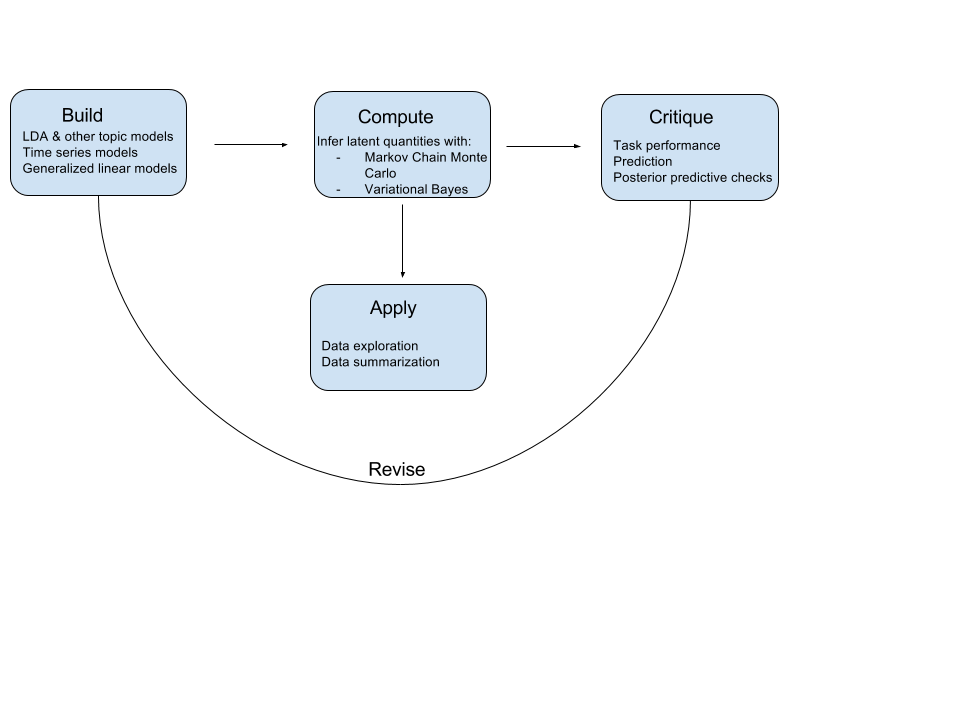
\includegraphics{box-blei-loop.png}
\caption{Iterative process for building, computing, critiquing, and applying topic models.\label{fig:box}}
\end{figure}

The perspective that guides our data analysis is based on ideas of the
University of Wisconsin-Madison statistician George Box and coworkers
{[}box1962useful{]}. D. M. Blei (2014) uses the ideas of Box and
colleagues in the specific case of iterative refinement of topic models.
Box (1976) articulated a process of scientific inquiry and statistical
collaboration in which scientists put forth a hypothesis about the
natural world, and, with assistance and guidance from statisticians,
design experiments to test the scientific hypothesis. After statistical
analysis of the experimental data, the scientific hypothesis is refined,
which leads to design and implementation of another experiment, and the
iterative process between scientific hypothesis and experiment
continues. Box (1976) also suggested that a statistician, working in
collaboration with scientists, might use scientific questions as
motivation to develop new statistical methods in experimental design and
data analysis. In this sense, there is a second iterative loop by which
a statistical researcher develops novel statistical methods because of
their immediate need to answer a scientific research question.

D. M. Blei (2014) adapts these iterative processes to the case of latent
variable models, such as LDA and other topic models. He argues that we
view the use of a topic model for a specific data analysis task as an
iterative procedure in which one proposes a simple topic model for the
data analysis, fits the model, interprets the results, and then, if
needed, refines the topic model with the goal of achieving data analysis
results that are more consistent with the research goals.

A critical step in this process is that of model critiquing. D. M. Blei
(2014) suggests using posterior predictive checks, evaluating
performance of desired tasks, and considering prediction performance in
this step. Recent research (Mimno \& Blei, 2011) has made progress in
developing methods for this last step in the iterative process
articulated by D. M. Blei (2014).

\section{Latent Dirichlet Allocation}\label{latent-dirichlet-allocation}

D. M. Blei et al. (2003) introduced LDA as a (generative) statistical
model in 2003. Although others had described similar statistical models
(Pritchard et al., 2000), D. M. Blei et al. (2003) first applied the
statistical model to text analysis. As we noted above, researchers in a
wide range of disciplines - including genetics, linguistics, psychology,
political science, and others - have enthusiastically adopted LDA and
related models to further their research efforts.

As D. M. Blei (2012) writes, the key to understanding LDA is to
recognize that a given document - be it a research article, a novel, or
a blog post - exhibits multiple topics. Each topic, in turn, is, in a
technical sense, a probability distribution over words. For example, a
topic related to evolution may heavily weight the words ``evolution'',
``evolutionary'', ``biology'', ``phylogenetic'', and ``species''. In a
given collection of documents, which we term a ``corpus'' of documents,
we assume that relatively few topics - on the order of 10 to 50 for most
analyses - are present.

LDA models have a hiearchical structure in which words make up
documents, and a collection of documents is a corpus. The corpus is
assumed to have (unobserved) topics, or themes. The purposes of LDA,
then, are to discover the unobserved topics from the texts and to
characterize documents by the topics that they contain.

\subsection{LDA Assumptions}\label{lda-assumptions}

One key assumption is often called the ``bag of words'' assumption. It
states that the order of words (and the order of topics) in documents
isn't important. Rather, we think of the process of generating words in
a document as a matter of first choosing a probability distribution over
topics, then, for each word in the document, using the selected
probability distribution over topics to choose a topic, and then
choosing a word from the corresponding probability distribution over the
vocabulary. Hence, we allow for documents to reflect multiple topics and
for each document to contain topics distinct proportions. Those familiar
with probability theory will recognize the ``bag of words'' assumption
as a statement of what probabilists call ``exchangeability''.

Hidden structures play key roles in LDA. While documents and their words
are observed, there remain three levels of hidden structures. The
topics, the per-document topic distributions, and the per-document,
per-word topic assignments constitute the unobserved variables that are
the goal of our inference procedures. In other words, our statistical
challenge, when working with topic models, is to use the observed
structures - documents and their words - to infer the three types of
hidden structures.

LDA's flexibility and adaptability have reduced the impact of its
initial limitations. In the last decade, researchers have devised
extensions of LDA, such as ``dynamic topic models'', that enable one to
model topic evolution over time(D. M. Blei \& Lafferty, 2006). Other
extensions of LDA attempt to account for correlations among topics (D.
M. Blei \& Lafferty, 2007, Li \& McCallum (2006)).

\section{LDA with print media}\label{lda-with-print-media}

Fitting LDA and related models of print media enables the user to
discover topics. Let's suppose that we want to understand the themes
that appear in a collection of print media articles. One strategy is to
read every article in the collection. We could then assign one or more
themes to each article and, at the end of our analysis, we would have a
collection of themes. However, an alternative approach, in keeping with
the theme-browsing ideas of D. M. Blei (2012), is to use LDA to identify
topics, which we treat as themes, in the collection of articles.

To demonstrate our topic modeling approach to discovering themes, or
topics, in print media, we used the Lexis Nexis Academic database to
acquire 746 New York Times (print) articles from March 19, 20, and 21 of
2016.

We loaded the raw downloaded text files into a computer program called
R, then partitioned the files into the 746 articles. To each article, we
applied a series of text processing steps. We split each article into
its distinct words and removed white space and punctuation before
converting all text to lower-case. At this stage, we had a collection of
words for each of the 746 distinct articles. After removing words that
occurred fewer than three times in the collection of articles and those
that appeared on our ``stop list'' of syntactical short words, including
articles and prepositions. With the remaining words, we created the
document-term matrix. The document-term matrix is much like an Excel
spreadsheet, where each row represents a document from the corpus and
each column represents a word from the vocabulary. The cells in the
matrix contain the number of times that each word appears in each
document. Entering the document-term matrix into a computer program (R),
we fit an LDA model with 20 topics.

\section{LDA with social media}\label{lda-with-social-media}

We downloaded tweets from the Twitter streaming API on the same three
consecutive days (March 19, 20, 21 in 2016). Due to the large volume of
downloaded tweets, we limited study to a one-hour period on each day
(approximately 12pm Central time to 1pm Central time). The downloaded
tweets constitute approximately one percent of all tweets during the
selected time periods, according to Twitter's documentation. We then
removed tweets that were in languages other than English, which left us
with a total of 193211 tweets.

At this point, we made an important modeling decision in which we
decided to treat each tweet as an independent document. This was an
important decision because tweets are forced, by Twitter, to be short
(no more than 140 characters in length). Because of their short length,
it may be incomplete to think of a single tweet as a full document. Yet,
as we'll see in the Results section, the model fitting yielded
interpretable topics.

Processing our tweets requires removal of punctuation, URLs, and
graphical characters that appear in tweets. After completing that step,
we divided each tweet into its words and fit LDA models. As with the
print media analysis, we chose to fit topic models with 20 topics.

\section{Inference in topic models}\label{inference-in-topic-models}

Existing strategies for fitting topic models can be divided into two
classes: 1. variational Bayes methods and 2. sampling methods.
Variational Bayes methods try to approximate the posterior probability
distribution by using optimization strategies from computer science.
Alternatively, sampling methods, such as those based on Markov chain
monte carlo (MCMC) approaches, draw samples from (an approximation to)
the posterior probability distribution and work with those samples to
approximate model parameters.

Computational implementations of both classes of strategies are freely
available. We include R computing code in the appendix.

\section{Interpreting results of topic
modeling}\label{interpreting-results-of-topic-modeling}

Statistical inference for topic models yields estimates for topics
(i.e., probability distributions over words), assignments of words
(within documents) to topics, and weights of topics in each document.
However, the user must impose meaning on the topics. For instance, a
topic may put heavy weights on the words ``genetics'', ``gene'',
``regulation'', ``DNA'', ``transcription'', and ``RNA''. The data
analyst needs to identify the similarities among these words - namely,
that they describe concepts related to genetics and molecular biology.
Fortunately, topic modeling procedures often discover topics that can be
summarized in one or two words once the data analyst has inspected the
most heavily weighted terms (for a given topic).

\section{Visualizing topic models}\label{visualizing-topic-models}

Visualizing topic modeling results is an active area of research. We
present below strategies that involve static and interactive displays.
Word clouds are a widely used method for presenting topic modeling
results. Unfortunately, the standard approach requires a distinct word
cloud for each topic. For models with more than ten topics, manually
examining wordclouds becomes unwieldy.

Word cloud construction is straightforward and implemented with freely
available software, such as the R package ``wordcloud''. For a single
topic, the default method for creating a word cloud involves the
identification of the most heavily weighted words in the topic. The user
may choose to assign font sizes that are proportional to the weights of
each word.

One newly developed method, which is implemented in the LDAvis R package
(Sievert \& Shirley, 2015), uses a singular value decomposition of the
fitted document-topic matrix to calculate principal components. Each
topic is then plotted in two dimensions, where the axes represent the
first two principal components. The LDAvis R package enhances this
second approach by making the figures interactive with D3 javascript.

For our analyses of tweets and New York Times articles, we created
wordclouds for each topic in the resulting models.

\section{Results from New York Times Articles
Analysis}\label{results-from-new-york-times-articles-analysis}

Examination of the resulting word clouds demonstrates that LDA is able
to discover coherent themes from a text corpus. We see that our
wordcloud in Figure \ref{fig:wc1} contains words, such as ``ballet'',
``song'', ``music'', and ``film'', that constitute the theme that we can
label as ``entertainment''. The wordcloud in Figure \ref{fig:wc2} may be
less clearly exhibiting a coherent theme, but it does contain a number
of words, such as ``boat'', ``river'', ``expedition'', related to travel
\& adventure. Figure \ref{fig:wc3} is difficult to interpret. On the one
hand, it contains ``books'', ``review'', and ``story'', which might
suggest a literature theme, but at the same time it contains a
collection of numbers. Figure \ref{fig:wc4} forms a cohesive collection
of words about sports.

\begin{figure}
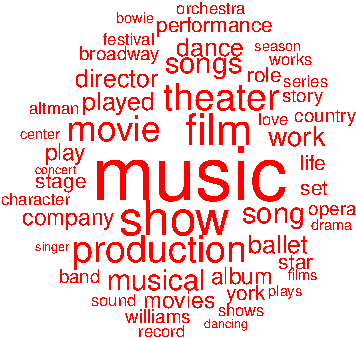
\includegraphics[width=\textwidth]{lda-tutorial-2016_files/figure-latex/wordcloud1-1.pdf}
\caption{Wordcloud for one topic from a 20-topic model of 746 New York Times articles. Larger font size corresponds to greater weight of that word in this topic.\label{fig:wc1}}
\end{figure}

\begin{figure}
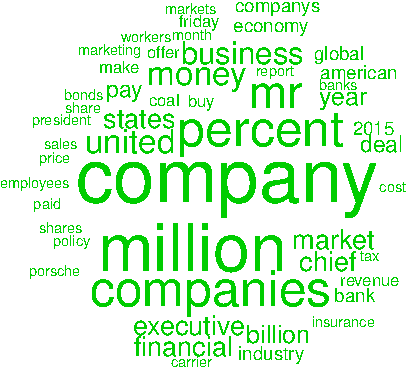
\includegraphics[width=\textwidth]{lda-tutorial-2016_files/figure-latex/wordcloud1-2.pdf}
\caption{Wordcloud for one topic from a 20-topic model of 746 New York Times articles. Larger font size corresponds to greater weight of that word in this topic.\label{fig:wc2}}
\end{figure}

\begin{figure}
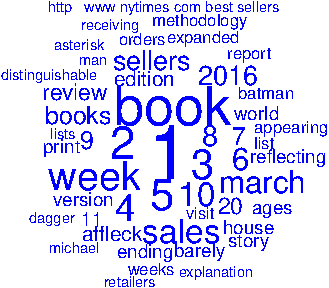
\includegraphics[width=\textwidth]{lda-tutorial-2016_files/figure-latex/wordcloud1-3.pdf}
\caption{Wordcloud for one topic from a 20-topic model of 746 New York Times articles. Larger font size corresponds to greater weight of that word in this topic.\label{fig:wc3}}
\end{figure}

\begin{figure}
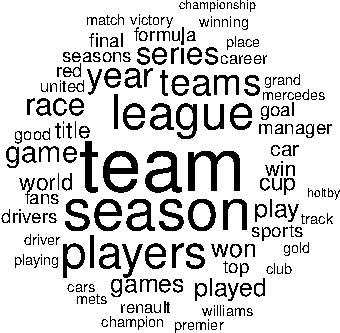
\includegraphics[width=\textwidth]{lda-tutorial-2016_files/figure-latex/wordcloud1-4.pdf}
\caption{Wordcloud for one topic from a 20-topic model of 746 New York Times articles. Larger font size corresponds to greater weight of that word in this topic.\label{fig:wc4}}
\end{figure}

\section{Results from Tweets
Analysis}\label{results-from-tweets-analysis}

\begin{figure}
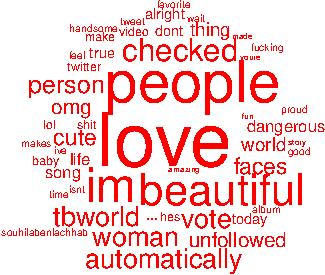
\includegraphics[width=\textwidth]{lda-tutorial-2016_files/figure-latex/tw-wordcloud1-5.pdf}
\caption{Wordcloud for one topic from a 20-topic model of 193,211 tweets. Larger font size corresponds to greater weight of that word in this topic.\label{fig:twc1}}
\end{figure}

\begin{figure}
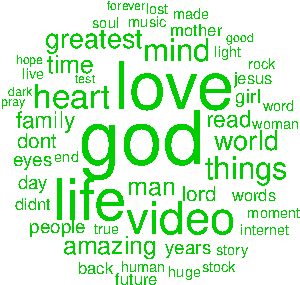
\includegraphics[width=\textwidth]{lda-tutorial-2016_files/figure-latex/tw-wordcloud1-2.pdf}
\caption{Wordcloud for one topic from a 20-topic model of 193,211 tweets. Larger font size corresponds to greater weight of that word in this topic.\label{fig:twc2}}
\end{figure}

\begin{figure}
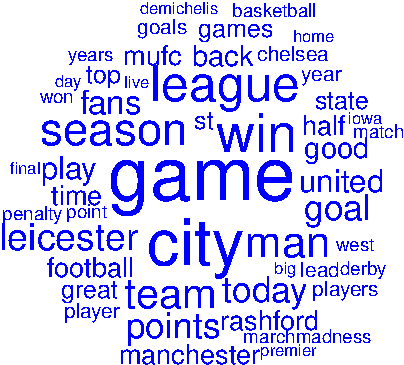
\includegraphics[width=\textwidth]{lda-tutorial-2016_files/figure-latex/tw-wordcloud1-3.pdf}
\caption{Wordcloud for one topic from a 20-topic model of 193,211 tweets. Larger font size corresponds to greater weight of that word in this topic.\label{fig:twc3}}
\end{figure}

\begin{figure}
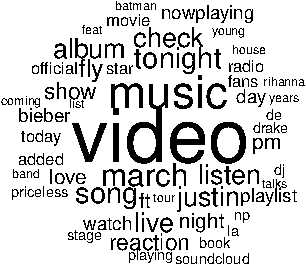
\includegraphics[width=\textwidth]{lda-tutorial-2016_files/figure-latex/tw-wordcloud1-4.pdf}
\caption{Wordcloud for one topic from a 20-topic model of 193,211 tweets. Larger font size corresponds to greater weight of that word in this topic.\label{fig:twc4}}
\end{figure}

\section{Discussion}\label{discussion}

We have presented preliminary results of our analysis of New York Times
articles and tweets from March 19, 20, and 21, 2016. Looking back at
Figure \ref{fig:box}, we see that we've omitted the model critiquing
step (D. M. Blei, 2014). Despite this, we still managed to discover
meaningful topics in both the tweets and the New York Times articles
with our initial models. Development of model critiquing strategies is
one of our immediate research goals.

\section{Future directions}\label{future-directions}

Analysis of new data sources and structures often requires development
of new statistical and computational methods. Topic models, despite
their newness, have already contributed to scholarly pursuits in a wide
range of social science, science, and humanities disciplines. Topic
model-based analyses in journalism and communications research provide a
practical method for summarizing and exploring the vast array of textual
data that we encounter. Furthermore, analysis with topic models
complements close reading and human annotation of texts. To fully
realize the potential of topic modeling in communications research, we
need to characterize the extent to which manual annotation of texts
coincides with topic model-based annotation of texts. When such
foundations are laid, we will realize a useful version of a topic-based
browser for texts, as D. M. Blei (2012) envisions.

\section{Online resources}\label{online-resources}

David Mimno, a Cornell University scholar, curates an annotated
bibliography of topic modeling research(Mimno, 2016). His bibliography
is available at this url:
\url{http://mimno.infosci.cornell.edu/topics.html}

\section{Computational implementation of LDA with
R}\label{computational-implementation-of-lda-with-r}

We present below code for using LDA (with a collapsed Gibbs sampler) in
the R statistical computing language (R Core Team, 2015).

\begin{Shaded}
\begin{Highlighting}[]
\KeywordTok{library}\NormalTok{(knitr)}
\NormalTok{opts_chunk$}\KeywordTok{set}\NormalTok{(}\DataTypeTok{echo =} \OtherTok{FALSE}\NormalTok{, }\DataTypeTok{message =} \OtherTok{FALSE}\NormalTok{, }\DataTypeTok{warning =} \OtherTok{FALSE}\NormalTok{, }
    \DataTypeTok{cache =} \OtherTok{TRUE}\NormalTok{, }\DataTypeTok{tidy =} \OtherTok{TRUE}\NormalTok{, }\DataTypeTok{tidy.opts =} \KeywordTok{list}\NormalTok{(}\DataTypeTok{blank =} \OtherTok{FALSE}\NormalTok{, }
        \DataTypeTok{width.cutoff =} \DecValTok{60}\NormalTok{))  }\CommentTok{# hide source code in the document}
\NormalTok{tx1 <-}\StringTok{ }\KeywordTok{scan}\NormalTok{(}\DataTypeTok{file =} \StringTok{"data/The_New_York_Times2016-03-21_17-02.TXT"}\NormalTok{, }
    \DataTypeTok{what =} \StringTok{"character"}\NormalTok{, }\DataTypeTok{blank.lines.skip =} \OtherTok{TRUE}\NormalTok{, }\DataTypeTok{sep =} \StringTok{"}\CharTok{\textbackslash{}n}\StringTok{"}\NormalTok{, }
    \DataTypeTok{encoding =} \StringTok{"UTF-8"}\NormalTok{, }\DataTypeTok{skipNul =} \OtherTok{TRUE}\NormalTok{)}
\NormalTok{tx2 <-}\StringTok{ }\KeywordTok{scan}\NormalTok{(}\DataTypeTok{file =} \StringTok{"data/The_New_York_Times2016-03-21_17-04.TXT"}\NormalTok{, }
    \DataTypeTok{what =} \StringTok{"character"}\NormalTok{, }\DataTypeTok{blank.lines.skip =} \OtherTok{TRUE}\NormalTok{, }\DataTypeTok{sep =} \StringTok{"}\CharTok{\textbackslash{}n}\StringTok{"}\NormalTok{, }
    \DataTypeTok{encoding =} \StringTok{"UTF-8"}\NormalTok{, }\DataTypeTok{skipNul =} \OtherTok{TRUE}\NormalTok{)}
\NormalTok{tx <-}\StringTok{ }\KeywordTok{c}\NormalTok{(tx1, tx2)}
\KeywordTok{library}\NormalTok{(wordtools)  }\CommentTok{#load R package 'wordtools'}
\NormalTok{tx_list <-}\StringTok{ }\KeywordTok{split_tx}\NormalTok{(}\DataTypeTok{tx =} \NormalTok{tx, }\DataTypeTok{patt =} \StringTok{"Copyright 20"}\NormalTok{)}
\KeywordTok{library}\NormalTok{(stringr)}
\NormalTok{tx_list2 <-}\StringTok{ }\KeywordTok{sapply}\NormalTok{(}\DataTypeTok{FUN =} \NormalTok{function(x) x[-(}\DecValTok{1}\NormalTok{:}\KeywordTok{which}\NormalTok{(}\KeywordTok{str_detect}\NormalTok{(}\DataTypeTok{string =} \NormalTok{x, }
    \DataTypeTok{pattern =} \StringTok{"LENGTH"}\NormalTok{)))], }\DataTypeTok{X =} \NormalTok{tx_list)}
\NormalTok{myfun <-}\StringTok{ }\NormalTok{function(x, }\DataTypeTok{pattern =} \StringTok{"Web Blog"}\NormalTok{) \{}
    \NormalTok{collapsed <-}\StringTok{ }\KeywordTok{paste}\NormalTok{(x, }\DataTypeTok{collapse =} \StringTok{" "}\NormalTok{)}
    \NormalTok{!stringr::}\KeywordTok{str_detect}\NormalTok{(collapsed, }\DataTypeTok{pattern =} \NormalTok{pattern)}
\NormalTok{\}}
\NormalTok{indswb <-}\StringTok{ }\KeywordTok{sapply}\NormalTok{(}\DataTypeTok{FUN =} \NormalTok{myfun, }\DataTypeTok{X =} \NormalTok{tx_list2)}
\NormalTok{indsurl <-}\StringTok{ }\KeywordTok{sapply}\NormalTok{(}\DataTypeTok{FUN =} \NormalTok{myfun, }\DataTypeTok{pattern =} \StringTok{"URL"}\NormalTok{, }\DataTypeTok{X =} \NormalTok{tx_list2)}
\KeywordTok{library}\NormalTok{(magrittr)}
\NormalTok{good_art <-}\StringTok{ }\NormalTok{tx_list2[indswb] %>%}\StringTok{ }\KeywordTok{sapply}\NormalTok{(}\DataTypeTok{FUN =} \NormalTok{function(x) \{}
    \NormalTok{x[-(}\KeywordTok{which}\NormalTok{(}\KeywordTok{str_detect}\NormalTok{(x, }\StringTok{"URL"}\NormalTok{)):}\KeywordTok{length}\NormalTok{(x))]}
\NormalTok{\})}
\KeywordTok{library}\NormalTok{(tm)}
\NormalTok{stopwords <-}\StringTok{ }\KeywordTok{c}\NormalTok{(tm::}\KeywordTok{stopwords}\NormalTok{(}\StringTok{"SMART"}\NormalTok{), }\StringTok{"dr"}\NormalTok{, }\StringTok{"mr"}\NormalTok{, }\StringTok{"ms"}\NormalTok{, }\StringTok{"mrs"}\NormalTok{)  }\CommentTok{# add titles to stoplist}
\NormalTok{good2 <-}\StringTok{ }\KeywordTok{sapply}\NormalTok{(}\DataTypeTok{FUN =} \NormalTok{function(x) }\KeywordTok{paste}\NormalTok{(x, }\DataTypeTok{collapse =} \StringTok{" "}\NormalTok{), }\DataTypeTok{X =} \NormalTok{good_art) %>%}\StringTok{ }
\StringTok{    }\NormalTok{stringr::}\KeywordTok{str_split}\NormalTok{(}\DataTypeTok{pattern =} \StringTok{" "}\NormalTok{) %>%}\StringTok{ }\KeywordTok{sapply}\NormalTok{(}\DataTypeTok{FUN =} \NormalTok{function(x) }\KeywordTok{gsub}\NormalTok{(}\StringTok{"'"}\NormalTok{, }
    \StringTok{""}\NormalTok{, x)) %>%}\StringTok{ }\CommentTok{# remove apostrophes}
\KeywordTok{sapply}\NormalTok{(}\DataTypeTok{FUN =} \NormalTok{function(x) }\KeywordTok{gsub}\NormalTok{(}\StringTok{"[[:punct:]]"}\NormalTok{, }\StringTok{" "}\NormalTok{, x)) %>%}\StringTok{ }\CommentTok{# replace punctuation with space}
\KeywordTok{sapply}\NormalTok{(}\DataTypeTok{FUN =} \NormalTok{function(x) }\KeywordTok{gsub}\NormalTok{(}\StringTok{"[[:cntrl:]]"}\NormalTok{, }\StringTok{" "}\NormalTok{, x)) %>%}\StringTok{ }\CommentTok{# replace control characters with space}
\KeywordTok{sapply}\NormalTok{(}\DataTypeTok{FUN =} \NormalTok{function(x) }\KeywordTok{gsub}\NormalTok{(}\StringTok{"^[[:space:]]+"}\NormalTok{, }\StringTok{""}\NormalTok{, x)) %>%}\StringTok{ }\CommentTok{# remove whitespace at beginning of documents}
\KeywordTok{sapply}\NormalTok{(}\DataTypeTok{FUN =} \NormalTok{function(x) }\KeywordTok{gsub}\NormalTok{(}\StringTok{"[[:space:]]+$"}\NormalTok{, }\StringTok{""}\NormalTok{, x)) %>%}\StringTok{ }\CommentTok{# remove whitesp Get rid of hashtags}
\KeywordTok{sapply}\NormalTok{(}\DataTypeTok{FUN =} \NormalTok{function(x) }\KeywordTok{str_replace_all}\NormalTok{(x, }\StringTok{"#[a-z,A-Z]*"}\NormalTok{, }\StringTok{""}\NormalTok{)) %>%}\StringTok{ }
\StringTok{    }\CommentTok{# Get rid of references to other screennames}
\KeywordTok{sapply}\NormalTok{(}\DataTypeTok{FUN =} \NormalTok{function(x) }\KeywordTok{str_replace_all}\NormalTok{(x, }\StringTok{"@[a-z,A-Z]*"}\NormalTok{, }\StringTok{""}\NormalTok{)) %>%}\StringTok{ }
\StringTok{    }\KeywordTok{sapply}\NormalTok{(}\DataTypeTok{FUN =} \NormalTok{function(x) }\KeywordTok{tolower}\NormalTok{(x)) %>%}\StringTok{ }\KeywordTok{sapply}\NormalTok{(}\DataTypeTok{FUN =} \NormalTok{function(x) x[!(x ==}\StringTok{ }
\StringTok{    ""}\NormalTok{)]) %>%}\StringTok{ }\CommentTok{# remove elements that are ''}
\KeywordTok{sapply}\NormalTok{(}\DataTypeTok{FUN =} \NormalTok{function(x) x[!(x %in%}\StringTok{ }\NormalTok{stopwords)])}
\CommentTok{# remove stopwords from}
\CommentTok{# http://cpsievert.github.io/LDAvis/reviews/reviews.html}
\CommentTok{# compute the table of terms:}
\NormalTok{n_min <-}\StringTok{ }\DecValTok{3}
\NormalTok{term_table <-}\StringTok{ }\KeywordTok{table}\NormalTok{(}\KeywordTok{unlist}\NormalTok{(good2)) %>%}\StringTok{ }\KeywordTok{sort}\NormalTok{(}\DataTypeTok{decreasing =} \OtherTok{TRUE}\NormalTok{)}
\NormalTok{term_table <-}\StringTok{ }\NormalTok{term_table[term_table >=}\StringTok{ }\NormalTok{n_min]}
\NormalTok{vocab <-}\StringTok{ }\KeywordTok{names}\NormalTok{(term_table)}
\NormalTok{get_terms <-}\StringTok{ }\NormalTok{function(x) \{}
    \NormalTok{index <-}\StringTok{ }\KeywordTok{match}\NormalTok{(x, vocab)}
    \NormalTok{index <-}\StringTok{ }\NormalTok{index[!}\KeywordTok{is.na}\NormalTok{(index)]}
    \KeywordTok{rbind}\NormalTok{(}\KeywordTok{as.integer}\NormalTok{(index -}\StringTok{ }\DecValTok{1}\NormalTok{), }\KeywordTok{as.integer}\NormalTok{(}\KeywordTok{rep}\NormalTok{(}\DecValTok{1}\NormalTok{, }\KeywordTok{length}\NormalTok{(index))))}
\NormalTok{\}}
\NormalTok{documents <-}\StringTok{ }\KeywordTok{lapply}\NormalTok{(good2, get_terms)}
\CommentTok{# Compute some statistics related to the data set:}
\NormalTok{D <-}\StringTok{ }\KeywordTok{length}\NormalTok{(documents)  }\CommentTok{# number of documents }
\NormalTok{W <-}\StringTok{ }\KeywordTok{length}\NormalTok{(vocab)  }\CommentTok{# number of terms in the vocab}
\NormalTok{doc.length <-}\StringTok{ }\KeywordTok{sapply}\NormalTok{(documents, function(x) }\KeywordTok{sum}\NormalTok{(x[}\DecValTok{2}\NormalTok{, ]))  }\CommentTok{# number of tokens per document }
\NormalTok{N <-}\StringTok{ }\KeywordTok{sum}\NormalTok{(doc.length)  }\CommentTok{# total number of tokens in the data }
\NormalTok{term.frequency <-}\StringTok{ }\KeywordTok{as.integer}\NormalTok{(term_table)  }\CommentTok{# frequencies of terms in the corpus}
\CommentTok{# MCMC and model tuning parameters:}
\NormalTok{K <-}\StringTok{ }\DecValTok{20}
\NormalTok{G <-}\StringTok{ }\DecValTok{5000}
\NormalTok{alpha <-}\StringTok{ }\FloatTok{0.02}
\NormalTok{eta <-}\StringTok{ }\FloatTok{0.02}
\CommentTok{# Fit the model:}
\KeywordTok{library}\NormalTok{(lda)}
\KeywordTok{set.seed}\NormalTok{(}\DecValTok{2016} \NormalTok{-}\StringTok{ }\DecValTok{3} \NormalTok{-}\StringTok{ }\DecValTok{22}\NormalTok{)}
\NormalTok{fit1 <-}\StringTok{ }\KeywordTok{lda.collapsed.gibbs.sampler}\NormalTok{(}\DataTypeTok{documents =} \NormalTok{documents, }\DataTypeTok{K =} \NormalTok{K, }
    \DataTypeTok{vocab =} \NormalTok{vocab, }\DataTypeTok{num.iterations =} \NormalTok{G, }\DataTypeTok{alpha =} \NormalTok{alpha, }\DataTypeTok{eta =} \NormalTok{eta, }
    \DataTypeTok{initial =} \OtherTok{NULL}\NormalTok{, }\DataTypeTok{burnin =} \DecValTok{1000}\NormalTok{, }\DataTypeTok{compute.log.likelihood =} \OtherTok{TRUE}\NormalTok{)}
\KeywordTok{library}\NormalTok{(wordcloud)}
\NormalTok{for (i in }\DecValTok{1}\NormalTok{:K) \{}
    \NormalTok{cloud.data <-}\StringTok{ }\KeywordTok{sort}\NormalTok{(fit1$topics[i, ], }\DataTypeTok{decreasing =} \OtherTok{TRUE}\NormalTok{)[}\DecValTok{1}\NormalTok{:}\DecValTok{50}\NormalTok{]}
    \KeywordTok{wordcloud}\NormalTok{(}\KeywordTok{names}\NormalTok{(cloud.data), }\DataTypeTok{freq =} \NormalTok{cloud.data, }\DataTypeTok{scale =} \KeywordTok{c}\NormalTok{(}\DecValTok{3}\NormalTok{, }
        \FloatTok{0.1}\NormalTok{), }\DataTypeTok{min.freq =} \DecValTok{1}\NormalTok{, }\DataTypeTok{rot.per =} \DecValTok{0}\NormalTok{, }\DataTypeTok{random.order =} \OtherTok{FALSE}\NormalTok{, }
        \DataTypeTok{col =} \DecValTok{1} \NormalTok{+}\StringTok{ }\NormalTok{i%%}\DecValTok{4}\NormalTok{)}
\NormalTok{\}}
\NormalTok{tweet_dir <-}\StringTok{ "data/tweets/"}
\NormalTok{fns <-}\StringTok{ }\KeywordTok{dir}\NormalTok{(tweet_dir)}
\NormalTok{out <-}\StringTok{ }\KeywordTok{character}\NormalTok{(}\DecValTok{0}\NormalTok{)}
\NormalTok{for (file in fns) \{}
    \NormalTok{tmp <-}\StringTok{ }\KeywordTok{read.csv}\NormalTok{(}\KeywordTok{file.path}\NormalTok{(tweet_dir, file), }\DataTypeTok{stringsAsFactors =} \OtherTok{FALSE}\NormalTok{)}
    \NormalTok{out <-}\StringTok{ }\KeywordTok{rbind}\NormalTok{(out, tmp)}
\NormalTok{\}}
\NormalTok{tweets <-}\StringTok{ }\NormalTok{out[out$lang ==}\StringTok{ "en"}\NormalTok{, ]}
\NormalTok{tw_txt <-}\StringTok{ }\NormalTok{tweets$text}
\KeywordTok{library}\NormalTok{(stringr)}
\NormalTok{tw_words <-}\StringTok{ }\NormalTok{stringr::}\KeywordTok{str_split}\NormalTok{(tw_txt, }\DataTypeTok{pattern =} \StringTok{" "}\NormalTok{) %>%}\StringTok{ }\KeywordTok{sapply}\NormalTok{(}\DataTypeTok{FUN =} \NormalTok{function(x) x[!(x ==}\StringTok{ }
\StringTok{    ""}\NormalTok{)]) %>%}\StringTok{ }\CommentTok{# remove elements that are ''}
\KeywordTok{sapply}\NormalTok{(}\DataTypeTok{FUN =} \NormalTok{function(x) }\KeywordTok{gsub}\NormalTok{(}\StringTok{"&amp"}\NormalTok{, }\StringTok{""}\NormalTok{, x)) %>%}\StringTok{ }\KeywordTok{sapply}\NormalTok{(}\DataTypeTok{FUN =} \NormalTok{function(x) }\KeywordTok{gsub}\NormalTok{(}\StringTok{"(RT|via)((?:}\CharTok{\textbackslash{}\textbackslash{}}\StringTok{b}\CharTok{\textbackslash{}\textbackslash{}}\StringTok{W*@}\CharTok{\textbackslash{}\textbackslash{}}\StringTok{w+)+)"}\NormalTok{, }
    \StringTok{""}\NormalTok{, x)) %>%}\StringTok{ }\KeywordTok{sapply}\NormalTok{(}\DataTypeTok{FUN =} \NormalTok{function(x) }\KeywordTok{gsub}\NormalTok{(}\StringTok{"@}\CharTok{\textbackslash{}\textbackslash{}}\StringTok{w+"}\NormalTok{, }\StringTok{""}\NormalTok{, x)) %>%}\StringTok{ }
\StringTok{    }\KeywordTok{sapply}\NormalTok{(}\DataTypeTok{FUN =} \NormalTok{function(x) }\KeywordTok{gsub}\NormalTok{(}\StringTok{"[[:punct:]]"}\NormalTok{, }\StringTok{""}\NormalTok{, x)) %>%}\StringTok{ }
\StringTok{    }\KeywordTok{sapply}\NormalTok{(}\DataTypeTok{FUN =} \NormalTok{function(x) }\KeywordTok{gsub}\NormalTok{(}\StringTok{"[[:digit:]]"}\NormalTok{, }\StringTok{""}\NormalTok{, x)) %>%}\StringTok{ }
\StringTok{    }\KeywordTok{sapply}\NormalTok{(}\DataTypeTok{FUN =} \NormalTok{function(x) }\KeywordTok{gsub}\NormalTok{(}\StringTok{"[^[:graph:]]"}\NormalTok{, }\StringTok{""}\NormalTok{, x)) %>%}\StringTok{ }
\StringTok{    }\CommentTok{# is this right???}
\KeywordTok{sapply}\NormalTok{(}\DataTypeTok{FUN =} \NormalTok{function(x) }\KeywordTok{gsub}\NormalTok{(}\StringTok{"http}\CharTok{\textbackslash{}\textbackslash{}}\StringTok{w+"}\NormalTok{, }\StringTok{""}\NormalTok{, x)) %>%}\StringTok{ }\KeywordTok{sapply}\NormalTok{(}\DataTypeTok{FUN =} \NormalTok{function(x) }\KeywordTok{gsub}\NormalTok{(}\StringTok{"[ }\CharTok{\textbackslash{}t}\StringTok{]\{2,\}"}\NormalTok{, }
    \StringTok{""}\NormalTok{, x)) %>%}\StringTok{ }\KeywordTok{sapply}\NormalTok{(}\DataTypeTok{FUN =} \NormalTok{function(x) }\KeywordTok{gsub}\NormalTok{(}\StringTok{"^}\CharTok{\textbackslash{}\textbackslash{}}\StringTok{s+|}\CharTok{\textbackslash{}\textbackslash{}}\StringTok{s+$"}\NormalTok{, }
    \StringTok{""}\NormalTok{, x)) %>%}\StringTok{ }\KeywordTok{sapply}\NormalTok{(}\DataTypeTok{FUN =} \NormalTok{function(x) }\KeywordTok{str_replace_all}\NormalTok{(x, }\StringTok{" "}\NormalTok{, }
    \StringTok{""}\NormalTok{))}
\NormalTok{tw_words <-}\StringTok{ }\KeywordTok{sapply}\NormalTok{(}\DataTypeTok{X =} \NormalTok{tw_words, }\DataTypeTok{FUN =} \NormalTok{function(x) }\KeywordTok{str_replace}\NormalTok{(x, }
    \StringTok{"RT @[a-z,A-Z]*: "}\NormalTok{, }\StringTok{""}\NormalTok{)) %>%}\StringTok{ }\KeywordTok{sapply}\NormalTok{(}\DataTypeTok{FUN =} \NormalTok{function(x) }\KeywordTok{str_replace_all}\NormalTok{(x, }
    \StringTok{"#[a-z,A-Z]*"}\NormalTok{, }\StringTok{""}\NormalTok{)) %>%}\StringTok{ }\KeywordTok{sapply}\NormalTok{(}\DataTypeTok{FUN =} \NormalTok{function(x) }\KeywordTok{str_replace_all}\NormalTok{(x, }
    \StringTok{"@[a-z,A-Z]*"}\NormalTok{, }\StringTok{""}\NormalTok{)) %>%}\StringTok{ }\CommentTok{# remove whitesp}
\KeywordTok{sapply}\NormalTok{(}\DataTypeTok{FUN =} \NormalTok{function(x) }\KeywordTok{tolower}\NormalTok{(x)) %>%}\StringTok{ }\KeywordTok{sapply}\NormalTok{(}\DataTypeTok{FUN =} \NormalTok{function(x) x[!(x %in%}\StringTok{ }
\StringTok{    }\NormalTok{tm::}\KeywordTok{stopwords}\NormalTok{(}\StringTok{"SMART"}\NormalTok{))])}
\CommentTok{# remove stopwords remove 'rt' and ''}
\NormalTok{tw_words <-}\StringTok{ }\KeywordTok{sapply}\NormalTok{(}\DataTypeTok{X =} \NormalTok{tw_words, }\DataTypeTok{FUN =} \NormalTok{function(x) x[!(x %in%}\StringTok{ }
\StringTok{    }\KeywordTok{c}\NormalTok{(}\StringTok{""}\NormalTok{, }\StringTok{"rt"}\NormalTok{))])}
\CommentTok{# from http://cpsievert.github.io/LDAvis/reviews/reviews.html}
\CommentTok{# compute the table of terms:}
\NormalTok{n_min <-}\StringTok{ }\DecValTok{3}
\NormalTok{term_table <-}\StringTok{ }\KeywordTok{table}\NormalTok{(}\KeywordTok{unlist}\NormalTok{(tw_words)) %>%}\StringTok{ }\KeywordTok{sort}\NormalTok{(}\DataTypeTok{decreasing =} \OtherTok{TRUE}\NormalTok{)}
\NormalTok{term_table <-}\StringTok{ }\NormalTok{term_table[term_table >=}\StringTok{ }\NormalTok{n_min]}
\NormalTok{vocab <-}\StringTok{ }\KeywordTok{names}\NormalTok{(term_table)}
\NormalTok{get_terms <-}\StringTok{ }\NormalTok{function(x) \{}
    \NormalTok{index <-}\StringTok{ }\KeywordTok{match}\NormalTok{(x, vocab)}
    \NormalTok{index <-}\StringTok{ }\NormalTok{index[!}\KeywordTok{is.na}\NormalTok{(index)]}
    \KeywordTok{rbind}\NormalTok{(}\KeywordTok{as.integer}\NormalTok{(index -}\StringTok{ }\DecValTok{1}\NormalTok{), }\KeywordTok{as.integer}\NormalTok{(}\KeywordTok{rep}\NormalTok{(}\DecValTok{1}\NormalTok{, }\KeywordTok{length}\NormalTok{(index))))}
\NormalTok{\}}
\NormalTok{documents <-}\StringTok{ }\KeywordTok{lapply}\NormalTok{(tw_words, get_terms)}
\CommentTok{# Compute some statistics related to the data set:}
\NormalTok{D <-}\StringTok{ }\KeywordTok{length}\NormalTok{(documents)  }\CommentTok{# number of documents }
\NormalTok{W <-}\StringTok{ }\KeywordTok{length}\NormalTok{(vocab)  }\CommentTok{# number of terms in the vocab}
\NormalTok{doc.length <-}\StringTok{ }\KeywordTok{sapply}\NormalTok{(documents, function(x) }\KeywordTok{sum}\NormalTok{(x[}\DecValTok{2}\NormalTok{, ]))  }\CommentTok{# number of tokens per document }
\NormalTok{N <-}\StringTok{ }\KeywordTok{sum}\NormalTok{(doc.length)  }\CommentTok{# total number of tokens in the data }
\NormalTok{term.frequency <-}\StringTok{ }\KeywordTok{as.integer}\NormalTok{(term_table)  }\CommentTok{# frequencies of terms in the corpus}
\CommentTok{# MCMC and model tuning parameters:}
\NormalTok{K <-}\StringTok{ }\DecValTok{20}
\NormalTok{G <-}\StringTok{ }\DecValTok{5000}
\NormalTok{alpha <-}\StringTok{ }\FloatTok{0.02}
\NormalTok{eta <-}\StringTok{ }\FloatTok{0.02}
\CommentTok{# Fit the model:}
\KeywordTok{library}\NormalTok{(lda)}
\KeywordTok{set.seed}\NormalTok{(}\DecValTok{2016} \NormalTok{-}\StringTok{ }\DecValTok{3} \NormalTok{-}\StringTok{ }\DecValTok{22}\NormalTok{)}
\NormalTok{fit1 <-}\StringTok{ }\KeywordTok{lda.collapsed.gibbs.sampler}\NormalTok{(}\DataTypeTok{documents =} \NormalTok{documents, }\DataTypeTok{K =} \NormalTok{K, }
    \DataTypeTok{vocab =} \NormalTok{vocab, }\DataTypeTok{num.iterations =} \NormalTok{G, }\DataTypeTok{alpha =} \NormalTok{alpha, }\DataTypeTok{eta =} \NormalTok{eta, }
    \DataTypeTok{initial =} \OtherTok{NULL}\NormalTok{, }\DataTypeTok{burnin =} \DecValTok{1000}\NormalTok{, }\DataTypeTok{compute.log.likelihood =} \OtherTok{TRUE}\NormalTok{)}
\KeywordTok{library}\NormalTok{(wordcloud)}
\NormalTok{for (i in }\DecValTok{1}\NormalTok{:K) \{}
    \NormalTok{cloud.data <-}\StringTok{ }\KeywordTok{sort}\NormalTok{(fit1$topics[i, ], }\DataTypeTok{decreasing =} \OtherTok{TRUE}\NormalTok{)[}\DecValTok{1}\NormalTok{:}\DecValTok{50}\NormalTok{]}
    \KeywordTok{wordcloud}\NormalTok{(}\KeywordTok{names}\NormalTok{(cloud.data), }\DataTypeTok{freq =} \NormalTok{cloud.data, }\DataTypeTok{scale =} \KeywordTok{c}\NormalTok{(}\DecValTok{3}\NormalTok{, }
        \FloatTok{0.1}\NormalTok{), }\DataTypeTok{min.freq =} \DecValTok{1}\NormalTok{, }\DataTypeTok{rot.per =} \DecValTok{0}\NormalTok{, }\DataTypeTok{random.order =} \OtherTok{FALSE}\NormalTok{, }
        \DataTypeTok{col =} \DecValTok{1} \NormalTok{+}\StringTok{ }\NormalTok{i%%}\DecValTok{4}\NormalTok{)}
\NormalTok{\}}
\end{Highlighting}
\end{Shaded}

\section{LDA with statistical
terminology}\label{lda-with-statistical-terminology}

We can also describe LDA with more formal statistical terminology. We
let \(\beta_1, \beta_2, ..., \beta_K\) be the \(K\) topics, where each
\(\beta_k\) is a probability distribution over the vocabulary. Topic
weights (or proportions) we denote by \(\theta_d\) for the \(d^{th}\)
document. We let \(\theta_{d,k}\) be the topic proportion for topic
\(k\) in document \(d\). Topic assignments for the \(d^{th}\) document
are \(z_d\), where \(z_{d,n}\) is the topic assignment for the
\(n^{th}\) word in the \(d^{th}\) document. Observed words for the
\(d^{th}\) document are \(w_d\), where \(w_{d, n}\) is the \(n^{th}\)
word for the \(d^{th}\) document.

We then use the above notation to specify the joint probability
distribution for all variables in the model:

\[p(\beta_{1:K}, \theta_{1:D}, z_{1:D}, w_{1:D}) = \prod_{i = 1}^Kp(\beta_i)\prod_{d = 1}^Dp(\theta_d)\left( \prod_{n = 1}^N p(z_{d,n}|\theta_d)p(w_{d,n}|\beta_{1:K}, z_{d,n})\right)\]

The vertical bars in the last expressions denote conditional
probabilities. Note that the topic assignments \(z_{d,n}\) depend on the
document's topic proportions. Whatismore, the observed word \(w_{d,n}\)
has a probability distribution that depends on both the entire
collection of topics, \(\beta_{1:K}\), and the topic, \(z_{d,n}\),
assigned to that word.

\section*{References}\label{references}
\addcontentsline{toc}{section}{References}

\hypertarget{refs}{}
\hypertarget{ref-blei2012probabilistic}{}
Blei, D. M. (2012). Probabilistic topic models. \emph{Communications of
the ACM}, \emph{55}(4), 77--84.

\hypertarget{ref-blei2014build}{}
Blei, D. M. (2014). Build, compute, critique, repeat: Data analysis with
latent variable models. \emph{Annual Review of Statistics and Its
Application}, \emph{1}, 203--232.

\hypertarget{ref-blei2006dynamic}{}
Blei, D. M., \& Lafferty, J. D. (2006). Dynamic topic models. In
\emph{Proceedings of the 23rd international conference on machine
learning} (pp. 113--120). ACM.

\hypertarget{ref-blei2007correlated}{}
Blei, D. M., \& Lafferty, J. D. (2007). A correlated topic model of
science. \emph{The Annals of Applied Statistics}, 17--35.

\hypertarget{ref-blei2003latent}{}
Blei, D. M., Ng, A. Y., \& Jordan, M. I. (2003). Latent dirichlet
allocation. \emph{The Journal of Machine Learning Research}, \emph{3},
993--1022.

\hypertarget{ref-box1976science}{}
Box, G. E. (1976). Science and statistics. \emph{Journal of the American
Statistical Association}, \emph{71}(356), 791--799.

\hypertarget{ref-derose2014victorian}{}
DeRose, C., Roy, C., \& Boehm, F. (2014). Victorian eyes: Literary,
statistical, and artistic perspectives on victorian novels -- and
dickens's unfinished murder mystery. \emph{Significance}, \emph{11}(2),
40--43.

\hypertarget{ref-griffiths2004hierarchical}{}
Griffiths, D., \& Tenenbaum, M. (2004). Hierarchical topic models and
the nested chinese restaurant process. \emph{Advances in Neural
Information Processing Systems}, \emph{16}, 17.

\hypertarget{ref-grimmer2010bayesian}{}
Grimmer, J. (2010). A bayesian hierarchical topic model for political
texts: Measuring expressed agendas in senate press releases.
\emph{Political Analysis}, \emph{18}(1), 1--35.

\hypertarget{ref-hall2008studying}{}
Hall, D., Jurafsky, D., \& Manning, C. D. (2008). Studying the history
of ideas using topic models. In \emph{Proceedings of the conference on
empirical methods in natural language processing} (pp. 363--371).
Association for Computational Linguistics.

\hypertarget{ref-hofmann1999probabilistic}{}
Hofmann, T. (1999). Probabilistic latent semantic indexing. In
\emph{Proceedings of the 22nd annual international aCM sIGIR conference
on research and development in information retrieval} (pp. 50--57). ACM.

\hypertarget{ref-li2006pachinko}{}
Li, W., \& McCallum, A. (2006). Pachinko allocation: DAG-structured
mixture models of topic correlations. In \emph{Proceedings of the 23rd
international conference on machine learning} (pp. 577--584). ACM.

\hypertarget{ref-mimno2016topic}{}
Mimno, D. (2016). Topic modeling bibliography. Retrieved from
\url{http://mimno.infosci.cornell.edu/topics.html}

\hypertarget{ref-mimno2011bayesian}{}
Mimno, D., \& Blei, D. (2011). Bayesian checking for topic models. In
\emph{Proceedings of the conference on empirical methods in natural
language processing} (pp. 227--237). Association for Computational
Linguistics.

\hypertarget{ref-pritchard2000inference}{}
Pritchard, J. K., Stephens, M., \& Donnelly, P. (2000). Inference of
population structure using multilocus genotype data. \emph{Genetics},
\emph{155}(2), 945--959.

\hypertarget{ref-r2015}{}
R Core Team. (2015). \emph{R: A language and environment for statistical
computing}. Vienna, Austria: R Foundation for Statistical Computing.
Retrieved from \url{https://www.R-project.org/}

\hypertarget{ref-rosen2004author}{}
Rosen-Zvi, M., Griffiths, T., Steyvers, M., \& Smyth, P. (2004). The
author-topic model for authors and documents. In \emph{Proceedings of
the 20th conference on uncertainty in artificial intelligence} (pp.
487--494). AUAI Press.

\hypertarget{ref-roy2013victorian}{}
Roy, C., DeRose, C., \& Boehm, F. (2013). Victorian eyes. Retrieved from
\url{http://victorianeyes.com}

\hypertarget{ref-r-LDAvis}{}
Sievert, C., \& Shirley, K. (2015). \emph{LDAvis: Interactive
visualization of topic models}. Retrieved from
\url{https://CRAN.R-project.org/package=LDAvis}

\end{document}
